% Options for packages loaded elsewhere
\PassOptionsToPackage{unicode}{hyperref}
\PassOptionsToPackage{hyphens}{url}
\documentclass[
]{article}
\usepackage{xcolor}
\usepackage{amsmath,amssymb}
\setcounter{secnumdepth}{-\maxdimen} % remove section numbering
\usepackage{iftex}
\ifPDFTeX
  \usepackage[T1]{fontenc}
  \usepackage[utf8]{inputenc}
  \usepackage{textcomp} % provide euro and other symbols
\else % if luatex or xetex
  \usepackage{unicode-math} % this also loads fontspec
  \defaultfontfeatures{Scale=MatchLowercase}
  \defaultfontfeatures[\rmfamily]{Ligatures=TeX,Scale=1}
\fi
\usepackage{lmodern}
\ifPDFTeX\else
  % xetex/luatex font selection
\fi
% Use upquote if available, for straight quotes in verbatim environments
\IfFileExists{upquote.sty}{\usepackage{upquote}}{}
\IfFileExists{microtype.sty}{% use microtype if available
  \usepackage[]{microtype}
  \UseMicrotypeSet[protrusion]{basicmath} % disable protrusion for tt fonts
}{}
\makeatletter
\@ifundefined{KOMAClassName}{% if non-KOMA class
  \IfFileExists{parskip.sty}{%
    \usepackage{parskip}
  }{% else
    \setlength{\parindent}{0pt}
    \setlength{\parskip}{6pt plus 2pt minus 1pt}}
}{% if KOMA class
  \KOMAoptions{parskip=half}}
\makeatother
\usepackage{graphicx}
\makeatletter
\newsavebox\pandoc@box
\newcommand*\pandocbounded[1]{% scales image to fit in text height/width
  \sbox\pandoc@box{#1}%
  \Gscale@div\@tempa{\textheight}{\dimexpr\ht\pandoc@box+\dp\pandoc@box\relax}%
  \Gscale@div\@tempb{\linewidth}{\wd\pandoc@box}%
  \ifdim\@tempb\p@<\@tempa\p@\let\@tempa\@tempb\fi% select the smaller of both
  \ifdim\@tempa\p@<\p@\scalebox{\@tempa}{\usebox\pandoc@box}%
  \else\usebox{\pandoc@box}%
  \fi%
}
% Set default figure placement to htbp
\def\fps@figure{htbp}
\makeatother
\ifLuaTeX
  \usepackage{luacolor}
  \usepackage[soul]{lua-ul}
\else
  \usepackage{soul}
\fi
\setlength{\emergencystretch}{3em} % prevent overfull lines
\providecommand{\tightlist}{%
  \setlength{\itemsep}{0pt}\setlength{\parskip}{0pt}}
\usepackage{bookmark}
\IfFileExists{xurl.sty}{\usepackage{xurl}}{} % add URL line breaks if available
\urlstyle{same}
\hypersetup{
  hidelinks,
  pdfcreator={LaTeX via pandoc}}

\author{}
\date{}

\begin{document}

\textbf{\ul{Partie Physique}}

Je commence à nouveau par briser un mythe bien connu~: non il est
impossible de se trouver «~au pied~» d'un arc-en-ciel. Pourquoi
allez-vous me demander~? Tout simplement car cela n'est pas un «~objet~»
réel, c'est-à-dire qu'il «~n'existe~» pas physiquement. Un arc-en-ciel
résulte d'un effet optique causé par la réfraction de la lumière du
soleil par les gouttes d'eau de la pluie. C'est pour cela qu'il faut
nécessairement pluie et soleil pour en observer un.

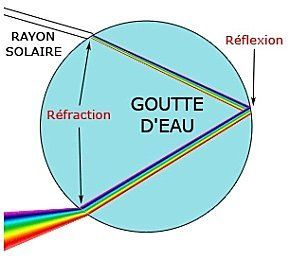
\includegraphics[width=3.025in,height=2.70833in,alt={Science - Comment se forme un arc en ciel}]{./media/image1.jpeg}Première
chose, comme vu précédemment, le soleil émet une lumière blanche
constitué de toutes les couleurs du spectre visible. On modélise une
goutte d'eau par une sphère comme ci-contre.

A l'arrivé d'un rayon a la surface d'une goutte, il va y avoir
réfraction a l'interface air-eau. Pour faire simple, l'air et l'eau sont
2 milieux ne possédant pas les mêmes propriétés et ainsi, la lumière va
changer de comportement lorsqu'elle passe de l'un à l'autre. En
particulier, la différence d'indice optique entre ces milieux induit une
séparation de la lumière blanche en toutes les couleurs de l'arc-en-ciel
comme montré ci-contre. Mais qu'est-ce que l'indice optique~? Il s'agit
d'une grandeur qui caractérise le fait que, dans un milieu qui n'est pas
le vide, la lumière se déplace à une vitesse v\textless c et que
celle-ci dépend du milieu. L'indice optique est le coefficient de
proportionnalité entre ces 2 vitesses et est donc caractéristique du
milieu de propagation de la lumière. Ainsi, la réfraction induit par la
goutte d'eau divise la lumière et cette lumière va aller se réfléchir
sur l'autre paroi de la goutte pour se réfracter de nouveau à la sortie
de celle-ci, ce qui accentue encore plus la division de la lumière. A
noter que la lumière peut subir plusieurs réflexions au sein de la
goutte d'eau ce qui peut engendrer les fameux «~double arc-en-ciel~» que
l'on peut observer certaines fois et pourrait même, en théorie, créer
plus d'arc-en-ciel lorsque les rayons subissent plus de 2 réflexions
dans la goutte. Ainsi, lorsque ce phénomène se produit sur un très grand
nombre de goutte, l'œil humain peut observer un arc-en-ciel. Il apparait
donc lorsque l'observateur regarde dans la direction opposée au soleil
et qu'un voile de goutte d'au se trouve dans l'air en face de
l'observateur.

L'apparition d'un arc-en-ciel n'est donc qu'un simple effet optique et
ne constitue pas un réel objet.

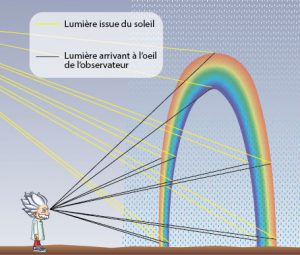
\includegraphics[width=3.125in,height=2.65833in,alt={Actualités météo: Comment se forment les arcs-en-ciel ? 22/05/2021}]{./media/image2.jpeg}

Si vous vous rapprochez de l'arc-en-ciel, soit il finira par disparaitre
car vos yeux ne recevront plus assez de rayon lumineux réfracté par les
gouttes, soit il vous paraitra avancer avec vous et vous ne pourrez donc
jamais l'atteindre. En effet, les calculs montrent que l'angle entre les
rayons arrivant de l'arc-en-ciel et la direction initiale des rayons du
soleil est de 42°, ainsi, l'arc-en-ciel parait avancé avec nous car son
rayon reste constant à nos yeux.

Illustrascience.fr, Comment se forme un arc-en-ciel,
\href{https://illustrascience.fr/comment-se-forme-un-arc-en-ciel/}{comment
se forme un arc en ciel ? - illustrascience}

\textbf{\ul{Partie Mathématiques et Équations}}

Prérequis~:

Lois de Descartes/Trigonométrie/Optique Géométrique

Scribd.com, Comprendre la formation de l'arc-en-ciel,
\href{https://fr.scribd.com/document/842974148/Optique-Arc-en-ciel}{Comprendre
la formation de l\textquotesingle arc-en-ciel \textbar{} PDF \textbar{}
Réfraction \textbar{} Arc en ciel}

On a 3 phénomènes à prendre en compte pour le calcul de D~:

Réfraction en entrée, réflexion, réfraction en sortie

On rappel les lois de Descartes de réfraction et réflexion~:

Réfraction~: \(n_{1}\sin{i_{1} = n_{2}\sin i_{2}}\)

Réflexion~: L'angle de réflexion est égal à l'angle d'incidence,
c'est-à-dire que le rayon réfléchi est symétrique par rapport à la
normale au dioptre.

Réfraction à l'entrée~: \(i - r\)

Réflexion~: \(\pi - 2r\)

Réfraction en sortie~: \(i - r\)

On a alors~:
\(\mathbf{D}\left( \mathbf{i} \right)\mathbf{= \pi + 2i - 4r}\)

La clé du problème réside maintenant dans le fait que l'arc en ciel est
observé pour la déviation correspondant au plus grand nombre de rayon
qui en ressortent donc la déviation minimale, ainsi, il faut
\(\frac{\mathbf{dD}}{\mathbf{di}}\mathbf{= 0}\) c'est-à-dire
\(\mathbf{2 - 4}\frac{\mathbf{dr}}{\mathbf{di}}\mathbf{= 0}\) donc
\(\frac{\mathbf{dr}}{\mathbf{di}}\mathbf{=}\frac{\mathbf{1}}{\mathbf{2}}\)

On différentie la relation de Descartes~:
\(n_{1}\sin{i_{1} = n_{2}\sin i_{2}}\) avec ici \(n_{1} = 1\),
\(i_{1} = i\), \(i_{2} = r\) donc

\[\mathbf{\cos}{\mathbf{i\ di = n}\mathbf{\cos}\mathbf{r\ dr}}
\]On a alors~:

\[\mathbf{\cos}{\mathbf{i = n\ cos\ r\ }\frac{\mathbf{dr}}{\mathbf{di}}\mathbf{=}\frac{\mathbf{n\cos r}}{\mathbf{2}}}\]

Or
\(\mathbf{\cos}^{\mathbf{2}}\mathbf{\theta + \ }\mathbf{\sin}^{\mathbf{2}}\mathbf{\theta = 1}\)
donc

\[\mathbf{\cos}^{\mathbf{2}}\mathbf{i =}\frac{\mathbf{n}^{\mathbf{2}}\mathbf{(1 -}\mathbf{\sin}^{\mathbf{2}}\mathbf{r)}}{\mathbf{4}}\mathbf{=}\frac{\mathbf{n}^{\mathbf{2}}\mathbf{(1 -}\frac{\mathbf{\sin}^{\mathbf{2}}\mathbf{i}}{\mathbf{n}^{\mathbf{2}}}\mathbf{)}}{\mathbf{4}}\mathbf{=}\frac{\mathbf{n}^{\mathbf{2}}\mathbf{-}\mathbf{\sin}^{\mathbf{2}}\mathbf{i}}{\mathbf{4}}\mathbf{=}\frac{\mathbf{n}^{\mathbf{2}}\mathbf{- 1 +}\mathbf{\cos}^{\mathbf{2}}\mathbf{i}}{\mathbf{4}}\mathbf{\ }\]

On obtient alors le résultat remarquable et remarqué~:

\[\mathbf{\cos}^{\mathbf{2}}\mathbf{i =}\frac{\mathbf{n}^{\mathbf{2}}\mathbf{- 1}}{\mathbf{3}}\]

On trouve alors que l'angle i tel que D est minimal est~:

\[\mathbf{i}_{\mathbf{D}}\mathbf{= \arccos}\sqrt{\frac{\mathbf{n}^{\mathbf{2}}\mathbf{- 1}}{\mathbf{3}}}\]

Pour l'eau, n=1.33 et on a alors~: \textbf{\hfill\break
}\[\mathbf{i}_{\mathbf{D}}\mathbf{= 59.6{^\circ}}\]

L'angle de réfraction correspondant est d'après la loi de Descartes~:

\[\mathbf{r}_{\mathbf{d}}\mathbf{=}\mathbf{\arcsin}\frac{\mathbf{\sin}\mathbf{i}_{\mathbf{d}}}{\mathbf{n}}\mathbf{= 40.4{^\circ}}\]

La valeur de la déviation est donc~:

\[\mathbf{D}_{\mathbf{\min}}\mathbf{= 180 + 119.2 - 161.6 = 137.6{^\circ}}\]

Ainsi l'angle entre la direction initiale des rayons solaires et les
rayons déviés est~:

\[\mathbf{\theta = 180 - 137.6 = 42.4{^\circ}}\]

On a donc bien démontré qu'un arc-en-ciel apparait avec un angle de 42°
entre la direction des rayons et ceux réfractés par les gouttes. Pour ce
qui est de la répartition des couleurs, on sait d'après la loi de Cauchy
que~:
\(n\left( \mathbf{\lambda} \right)\mathbf{= A +}\frac{\mathbf{B}}{\mathbf{\lambda}}\)
avec A et B des constantes.

Ainsi, les faibles longueurs d'ondes seront plus déviées et apparaitront
alors en dessous dans l'arc-en-ciel alors que les hautes seront moins
déviées et apparaitront au-dessus. C'est pourquoi le rouge apparait tout
en haut de l'arc alors que le violet se trouve tout en bas.
Typiquement~: \(\theta_{rouge} = 42.1{^\circ}\) alors que
\(\theta_{violet} = 40.6{^\circ}\)

On pourrait traiter le cas de l'arc en ciel secondaire mais les calculs
sont identiques à cela près que
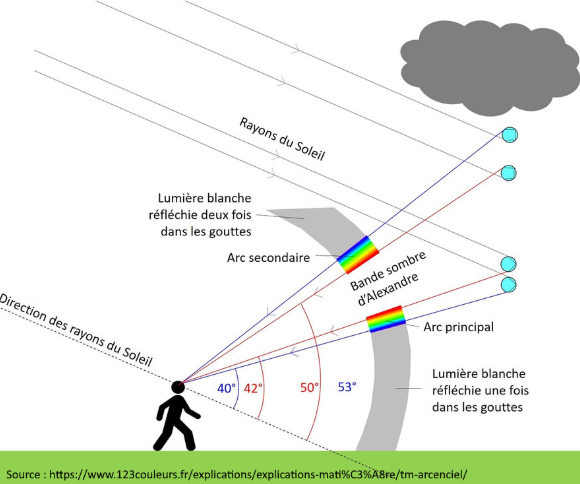
\includegraphics[width=2.68333in,height=2.29444in]{./media/image4.png}l'on
rajoute une réflexion et donc \(\pi - 2r\) a la déviation de la lumière
dans la goutte. Je laisse la joie au lecteur de suivre les exactes mêmes
étapes que précédemment avec la valeur de D qui convient et vous
trouverez les résultats qui sont répertoriés dans la figure ci-contre.
Les couleurs seront inversées par rapport à l'arc-en-ciel primaire à
cause de la seconde réflexion.

\end{document}
